\documentclass[a4paper, 10pt]{article}
\usepackage[a4paper, top = 1.5cm, bottom = 1.5cm, left = 1cm, right = 1cm]{geometry}
\usepackage{graphicx}
\usepackage{subcaption}
\usepackage{mathtools}
\usepackage{amsfonts}
\usepackage[english, russian]{babel}
\title{Лабораторная работа № 3.1.3 "Измерение магнитного поля Земли"}
\author{Кирилл Шевцов Б03-402}
\date{8.09.2025}
\begin{document}
\maketitle
\section*{Цель работы}
Исследовать свойства постоянных неодимовых магнитов, с их помощью измерить горизональную и вертикальную составляющую индукции магнитного поля Земли и наклонение.
\section*{Оборудование}
Неодимовые магниты, тонкая нить для изготовления крутильного маятника, медная проволока, электронные весы, секундомер, измеритель магнитной индукции, штангенциркуль.
\section*{Экспериментальная установка}
Следующие установки помогут измерить: период крутильных колебаний (\ref{sub@крутильный маятник}), силу отрыва цепочки шариков (\ref{sub@установка для силы отрыва}),
магнитный момент для двух шариков (\ref{sub@магнитный момент установка}).
\begin{figure}[htbp]
        \centering
        \begin{subfigure}{0.2\textwidth}
            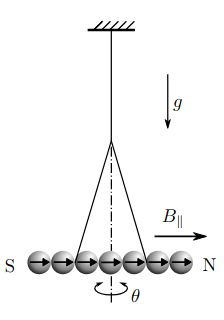
\includegraphics[width=\linewidth]{p1.png}
            \caption{крутильный маятник}
            \label{крутильный маятник}
        \end{subfigure}
        \hspace{2cm}
        \begin{subfigure}{0.2\textwidth}
            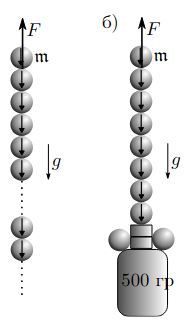
\includegraphics[width=\linewidth]{p2.png}
            \caption{установка для силы отрыва}
            \label{установка для силы отрыва}
        \end{subfigure}
        \hspace{2cm}
        \begin{subfigure}{0.2\textwidth}
            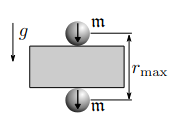
\includegraphics[width=\linewidth]{p3.png}
            \caption{измерение магнитного момента}
            \label{магнитный момент установка}
        \end{subfigure}
        \begin{subfigure}{0.2\linewidth}
            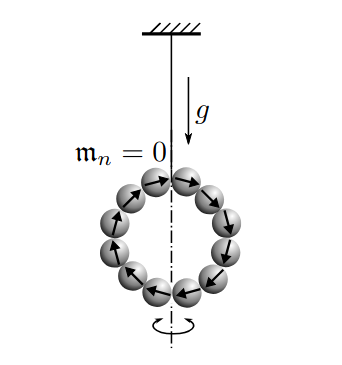
\includegraphics[width=\linewidth]{p4.png}
            \caption{стрелка, скрученная в кольцо}
            \label{стрелка, скрученная в кольцо}
        \end{subfigure}
        \caption{экспериментальные установки}
        \label{установки}
    \end{figure}\\
Установки \ref{sub@установка для силы отрыва} и \ref{sub@магнитный момент установка} дают один результат для измерения магнитного момента. Можно скрутить магнитную стрелку в кольцо, и
показать, что упругость нити при вычислении периода колебаний стрелки можно не учитывать (см. рис. \ref{sub@стрелка, скрученная в кольцо}).
\section*{Необходимые формулы и теория}
\paragraph{}
Простейший магнитный диполь может быть образован витком с током или постоянным магнитом.\\
Магнитное поле точечного диполя вычисляется подобно формуле напряженности электрического поля этого диполя:
\begin{equation}
    \mathbf{B} = \frac{\mu_{0}}{4 \pi}\left(\frac{3({\mathfrak{m}} \cdot \mathbf{r}) \mathbf{r}}{r^{5}} - \frac{{\mathfrak{m}}}{r^{3}}\right)
    \label{Магнитное поле диполя}
\end{equation}
Здесь $\mu_{0} = 4\pi \cdot 10^{-7}$ Гн/м - магнитная постоянная, $\mathbf{\mathfrak{m}}$ - магнитный момент точечного диполя, $\mathbf{r}$ - радиус вектор, направленный от диполя в рассматриваемую точку.\\
Во внешнем магнитном поле с индукцией $\mathbf{B}$ на точечный магнитный диполь $\mathfrak{m}$ действует механический момент сил:
\begin{equation}
    \mathbf{M} = [\mathfrak{m} \times \mathbf{B}]
    \label{Момент}
\end{equation}
В неоднородном магнитном поле на точечный диполь действует сила:
\begin{equation}
    \mathbf{F} = (\mathfrak{m} \cdot \nabla)\mathbf{B}
    \label{Сила действия на диполь}
\end{equation}
В частности, проекция силы на ось $\mathit{Ox}$:
\begin{equation}
    F_{x} = \mathfrak{m}_{x}\frac{\partial B_{x}}{\partial x} + \mathfrak{m}_{y}\frac{\partial B_{x}}{\partial y} + \mathfrak{m}_{z}\frac{\partial B_{x}}{\partial z}
    \label{Проекция силы}
\end{equation}
\paragraph{}
Формулы (\ref{Момент}) и (\ref{Сила действия на диполь}) помогают рассчитать силу взаимодействия магнитов с моментами $\mathfrak{m_{1}}$ и $\mathfrak{m_{2}}$ в рамках точечных диполей:
\begin{equation}
    F_{12} = \mathfrak{m}_{1}{\frac{\partial {B_{2}}}{\partial r}} = \mathfrak{m}_{1}\frac{\partial (2\mathfrak{m}_{2}/r^{3})}{\partial r}  =-6\frac{\mathfrak{m}_{1}\mathfrak{m}_{2}}{r^{4}}
    \label{Сила взаимодействия диполей}
\end{equation}
Еще одной характеристикой магнитов является намагниченность, равная объёмной плотности магнитного момента:
\begin{equation}
    \mathbf{M} = \mathfrak{m}/V
    \label{намагниченность}
\end{equation}
Вf\newline
Для рассчета магнитного поля Земли есть несколько методов:
\begin{enumerate}
    \item Определить магнитный момент $\mathfrak{m}$ двух из шариков, определив наибольшее расстояние $\mathit{r_{max}}$, на котором они смогут удерживать друг друга в поле тяжести. По величине $\mathfrak{m}$\
    с помощью (\ref{Магнитное поле диполя}) рассчитать величину индукции вблизи любой точки на поверхности шара радиусом $\mathit{R}$.
    \begin{equation}
        \mathfrak{m} = \sqrt{\frac{mgr_{max}^{4}}{6}}
        \label{Магнитный момент}
    \end{equation}
    Учтем, что здесь магнитный момент представлен вычислением в единицах СГС.
    \item Величину магнитного поля можно определить с помощью силы сцепления намагниченных шариков. Определим ее, как необходимую силу для разрыва двух сцепившихся шариков. Сила сцепления (\ref{Сила взаимодействия диполей}) равна:
    \begin{equation}
        F_{0} = \frac{6\mathfrak{m}^{2}}{(2R)^{4}} = \frac{3\mathfrak{m}^2}{8R^{4}}
        \label{Сила сцепления}
    \end{equation}
    Минимальный вес цепочки, при которой она оторвется от верхнего шарика, равна:
    \begin{equation}
        F = F_{0}\left(\sum_{k = 1}^n \frac{1}{k^{4}}\right) \approx 1,08F_{0}
        \label{Вес цепочки}
    \end{equation}
    Учтём, что сила сцепления шариков при их отрывании убывает как $1/r^{4}$.
    \item Рассчитать магнитное поле Земли можно с помощью составляющих: вертикальной и горизонтальной, ведь:
    \begin{equation}
        \vec{\mathbf{B}} = \vec{\mathbf{B_{||}}} + \vec{\mathbf{B_{\perp}}}
        \label{Векторная сумма полей}
    \end{equation}
    Горизонтальную составляющую поля можно рассчитать с помощью измерения периода крутильных колебаний ''магнитной стрелки'' вокруг своей оси:
    \begin{equation}
        T_{n} = 2\pi \sqrt{\frac{mR^{2}}{3\mathfrak{m}B_{||}}}\cdot n
        \label{Период крутильных колебаний}
    \end{equation}
    По зависимости $T(n) = f(n)$, а это прямая, можно определить коэффициент наклона и по нему найти модуль горизонтальной составляющей поля.\\
    Вертикальная составляющая: из-за возникающего момента силы натяжения нити необходимо
    выровнять положение стрелки, подвесив на некоторое ее расстояние $x$ груз массой $m_{x}$.Отсюда получим выражение для вертикальной составляющей магнитного поля:
    \begin{equation}
        m_{x}gx = n\mathfrak{m}B_{\perp} \iff B_{\perp} = \frac{m_{x}gx}{n\mathfrak{m}}
        \label{Вертикальная составляющая}
    \end{equation}
\end{enumerate}
\section*{Выполнение работы}
\begin{enumerate}
    \item Измерим массу одного шарика с помощью весов и его диаметр с помощью штангенциркуля (погрешности измерений массы и диаметра $\Delta m$, $\Delta d$), вычислим его объем:
    \begin{center}
    \begin{tabular}{|c|c|c|c|c|c|}
            \hline
            Масса шарика, г & Диаметр шарика, cm & $\Delta m$, г & $\Delta d$, cm & V, $cm^{3}$ & $\Delta V$, $cm^{3}$\\
            $0.841\pm 0.001$ & $0.59\pm 0.01$ & 0.001 & 0.01 & 0.022 & $2.23\cdot 10^{-3}$\\
            \hline
        \end{tabular}
    \end{center}
    \begin{equation*}
        V = \frac{1}{6}\pi D^{6} = 0.022\pm \ cm^{3} \quad \Delta V = \frac{6V\Delta D}{D} = 2.23\cdot 10^{-3} cm^{3}
    \end{equation*}
    \item Измерим магнитное поле на полюсах шарика с момощью магнитрометра: ${B_{p}}$ = $420\pm 1$ мТл. Магнитное поле неодимового магнита больше всего
    на его полюсах, где ориентирован магнитный момент.
    \item Рассчитаем величину магнитного момента одного шарика с помощью установки (\ref{sub@магнитный момент установка}). Максимальное
    расстояние, при котором шарики перестают взаимодействовать равно $r_{max} = 2.20\pm 0.05$ см
    \begin{align*}
        \mathfrak{m} = \sqrt{\frac{0.841\cdot 980.67\cdot 2.20^{4}}{6}} = 56.74\pm 0.85\ \text{эрг/Гс} \quad
        \Delta \mathfrak{m} = {\mathfrak{m}}\cdot \left(\frac{\Delta m}{2m} + \frac{2\Delta r_{max}}{r_{max}} + \frac{\Delta g}{2g}\right) = 0.85\ \text{эрг/Гс}
    \end{align*}
    \item Рассчитаем величину намагниченности $\mathbf{M}$ материала шариков и остаточную индукцию поля ${B_{r}}$ по формуле (\ref{намагниченность}).
    \begin{align*}
        \mathbf{M} = \frac{\mathfrak{m}}{V} = \frac{3\mathfrak{m}}{4\pi R^{3}} = 527.64\pm 61.39\ \text{Гс} & \quad \Delta \mathbf{M} = \mathbf{M}\left(\frac{\Delta \mathfrak{m}}{\mathfrak{m}} + \frac{\Delta V}{V}\right) = 61.39\ \text{Гс}\\
        {B_{r}} = 4\pi\mathbf{M} = 6630.47\pm 771.44\ \text{Гс} & \quad \Delta {B_{r}} = \frac{{B_{r}}\Delta \mathbf{M}}{\mathbf{M}} = 771.44\ \text{Гс}
    \end{align*}
    \item Остаточная индукция и индукция на полюсах магнита связаны соотношением: ${B_{p}} = \frac{2}{3}{B_{r}}$.\\ 
    Тогда ${B_{r}} = 3/2B_{p} = 630\pm 1\ \text{мТл} = 6300\ \text{Гс}$, ошибка рассчитанного в предыдущем пункте значения индукции относительно измеренного магнитрометром: $\varepsilon \sim 10^{-2}$. Это говорит о том, что
    поле на полюсах шарика было измерено верно (то есть там, где ориентирован магнитный момент) и предложенный магнитрометр в работе подходит для изучения магнитный свойств
    неодимового магнита.
    \item Скрутим магнитную стрелку в виде кольца, необходимо возбудить малые колебания колечки, период малых колебаний $T = 50\pm 1\ \text{с}$. Покажем, что при расчетах составляющих поля упругостью нити можно пренебречь:
    \begin{align*}
        f = \frac{(4\pi)^{2} I}{T^{2}} = \frac{16\pi^{2}}{2500}\cdot 6mR^{2} = 2.77\cdot 10^{-5}\ \text{Нм/рад} \quad \Delta f = f \left(\frac{\Delta m}{m} + \frac{\Delta D}{D} + \frac{2\Delta T}{T}\right) = 6.30\cdot 10^{-6}\ \text{Нм/рад}
    \end{align*}
    Поэтому жесткостью нити при колебаниях магнитной стрелки можно пренебречь.
    \item Исследуем зависимость периода крутильных колебаний от количества шариков, составляющих стрелку:
    \begin{center}
        \begin{tabular}{|c|c|c|c|c|c|c|c|c|c|c|}
            \hline
            Количество шариков $n$ & 3 & 4 & 5 & 6 & 7 & 8 & 9 & 10 & 11 & 12\\
            \hline
            Время $t$, с & 10.67 & 14.18 & 16.00 & 23.41 & 26.78 & 28.34 & 34.50 & 42.34 & 50.03 & 53.50\\
            Период $T = t/N$, с & 1.067 & 1.418 & 1.600 & 2.341 & 2.678 & 2.834 & 3.450 & 4.234 & 5.003 & 5.350\\
            \hline
            Число оборотов $N$ & \multicolumn{10}{|c|}{10}\\
            $\Delta t$, с & \multicolumn{10}{|c|}{0.01}\\
            $\Delta T$, с & \multicolumn{10}{|c|}{0.001}\\
            \hline
        \end{tabular}
    \end{center}
    Коэффициент регрессии графика $T(n)$ равен $k = 0.433\pm 0.029$ (см. рисунок \ref{графики моментов и периодов}).
    \item Исследуем зависимость момента силы тяжести $\mathcal{M}(n)$ от количества шариков в цепочке. Подвесим стрелку в положение равновесия, уравняем её дополнительным грузом. Используем четное число шариков в цепочке:
    \begin{center}
        \begin{tabular}{|c|c|c|c|c|c|}
            \hline
            Число шариков & 4 & 6 & 8 & 10 & 12\\
            Масса $m_{x}$, г & 0.41 & 0.20 & 0.23 & 0.20 & 0.16\\
            Длина плеча $l_{x}$, см & 0.59 & 1.18 & 1.77 & 2.36 & 2.95\\
            $\mathcal{M}_{n}$, г*см2/с2 & 237.06 & 335.36 & 383.18 & 462.65 & 462.56\\
            $\Delta \mathcal{M}_{n}$, г*см2/с2 & 3.3 & 3.0 & 2.8 & 3.1 & 4.1\\
            \hline
            $\Delta l_{x}$, см & \multicolumn{5}{|c|}{0.01}\\
            $\Delta m$, г & \multicolumn{5}{|c|}{0.01}\\
            \hline
        \end{tabular}
        \label{дополнительный груз для магнитной стрелки}
    \end{center}
    Коэффициент регрессии графика $\mathcal{M}(n)$ равен $k = 28.914\pm 4.624$ (см. рисунок \ref{графики моментов и периодов})
    \item Рассчитаем горизональную составляющую магнитного поля по полученному коэффициенту регрессии:
    \begin{align*}
        % \mathbf{B_{||}} = \frac{4\pi^{2} mR^{2}}{3\mathfrak{m}k^{2}} = 0.083\ \text{} \quad
        k & = 2\pi \sqrt{\frac{mR^{2}}{3\mathfrak{m}{B_{||}}}} \rightarrow {B_{||}} = \frac{4\pi^{2}mR^{2}}{3\mathfrak{m}k^{2}} = 0.091\pm 0.079\ \text{Гс}\\
        \Delta {B_{||}} & = {B_{||}}\left(\frac{\Delta m}{m} + \frac{2\Delta R}{R} - \frac{2\Delta k}{k} - \frac{\Delta \mathfrak{m}}{\mathfrak{m}}\right) = 0.079\ \text{Гс}
    \end{align*}
    \item Рассчитаем вертикальную составляющую магнитного поля по полученному коэффициенту регрессии:
    \begin{align*}
        % \mathbf{B_{\perp}} = \frac{k}{\mathfrak{m}} = 0.63\ \text{} \quad
        % \Delta \mathbf{B_{\perp}} = \mathbf{B_{\perp}}\left(\frac{\Delta k}{k} - \frac{\Delta \mathfrak{m}}{\mathfrak{m}}\right) = 0.22\ \text{}
        B_{\perp} = \frac{k}{\mathfrak{m}} = 0.50\pm 0.17\ \text{Гс} & \quad \Delta B_{\perp} = B_{\perp}\left(\frac{\Delta \mathfrak{m}}{\mathfrak{m}} + \frac{\Delta k}{k}\right) = 0.17\ \text{Гс}
    \end{align*}
    \item Рассчитаем величину магнитного наклонения:
    \begin{align*}
        \beta & = \arctan{\frac{{B_{\perp}}}{{B_{||}}}} = 79{.}68^\circ \pm 13{.}08^{\circ}\\
        \Delta \beta & = \sqrt{\left(\frac{B_{||}}{B_{\perp}^2 + B_{||}^2}\Delta B_{\perp}\right)^2 + \left(\frac{B_{\perp}}{B_{\perp}^2 + B_{||}^2}\Delta B_{||}\right)^2} = 13{.}08^{\circ}
    \end{align*}
    Полученное значение угла соответсвует наклонению широты Московского региона (значение варьируется в диапазоне $70^{\circ}-80^{\circ}$)
    \item Рассчитаем полную величину магнитного поля ${B}$:
    \begin{align*}
        {B} & = \sqrt{{B_{||}}^{2} + {B_{\perp}}^{2}} = 0.508\pm 0.187\ \text{Гс}\\
        \Delta {B} & = {B}\sqrt{\left(\frac{\partial {B}}{\partial {B_{||}}}\Delta {B_{||}}\right)^{2} + \left(\frac{\partial {B}}{\partial {B_{\perp}}}\Delta {B_{\perp}}\right)^{2}} = 0.187\ \text{Гс}
    \end{align*}
    Полученное значение магнитного поля соответсвует значению магнитного поля Земли (это диапазон значений 0.50-0.60 Гс).
\end{enumerate}
\section*{Графики для измеренных данных}
Представим визуализацию зависимостей данных, описанных в предыдущем параграфе.
\begin{figure}[htbp]
    \centering
    \begin{subfigure}{0.45\textwidth}
        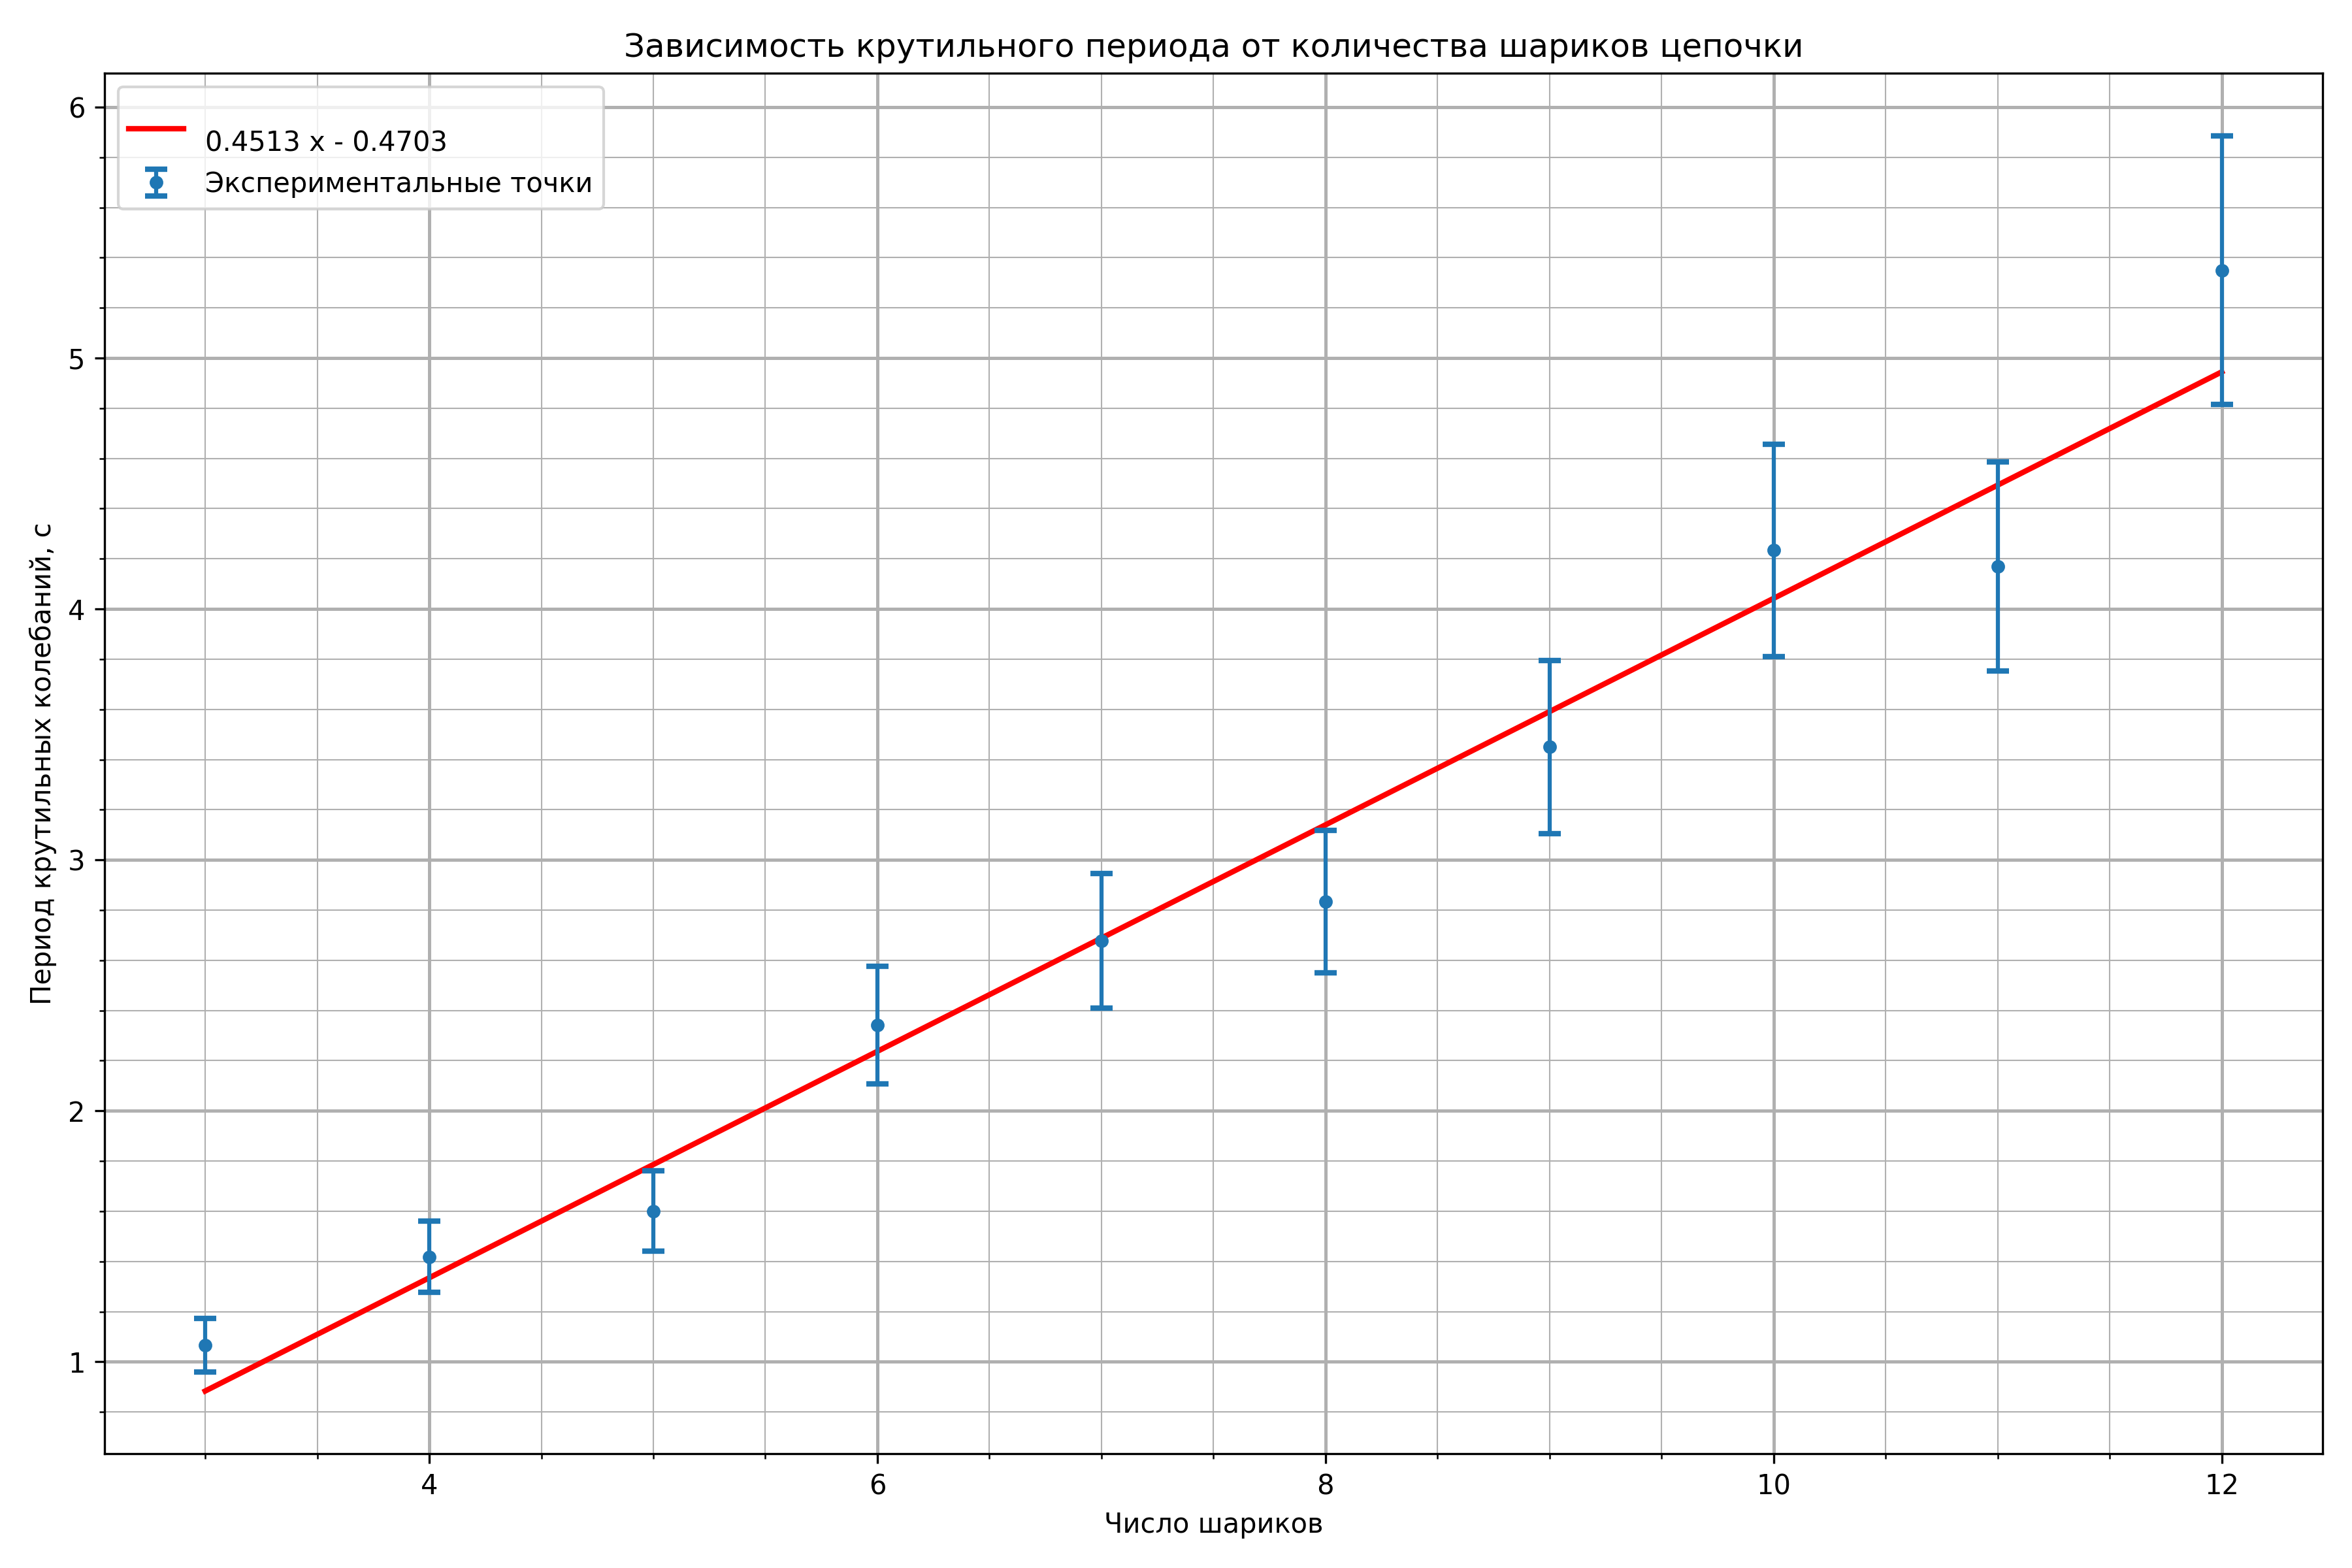
\includegraphics[width=\linewidth]{period.png}
        \caption{график крутильных колебаний стрелки}
        \label{горизонтальная составляющая}
    \end{subfigure}
    \begin{subfigure}{0.45\textwidth}
        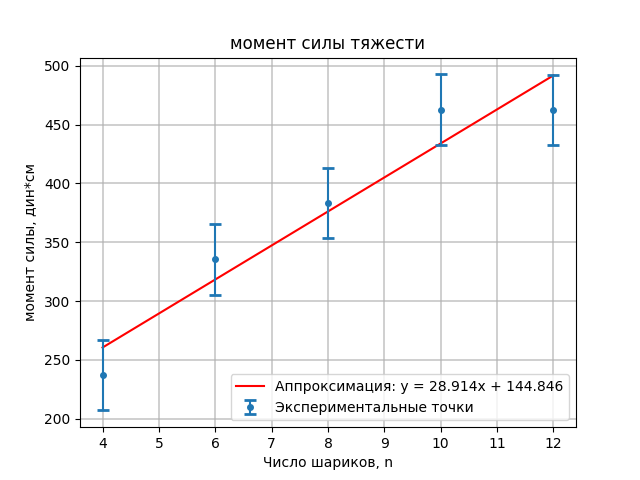
\includegraphics[width=\linewidth]{vertical.png}
        \caption{зависимость момента силы тяжести от числа шариков}
        \label{вертикальная составляющая}
    \end{subfigure}
    \caption{графики $T(n)$ и $\mathcal{M}(n)$}
    \label{графики моментов и периодов}
\end{figure}
\section*{Вывод}
    В работе были изучены свойства неодимовых магнитов, было измерено магнитное поле Земли, магнитное наклонение на широте Долгопрудного.
    \begin{enumerate}
        \item Неодимовые магниты хорошо подходят для изучения магнитных явлений, поскольку они обладают хорошей намагниченностью, даже самые
        маленькие кусочки обладают большой силой и магнитной энергией.
        \item Измеренное магнитное поле Земли измерено довольно точно к табличному значению, поэтому использовать неодимовые магниты для измерения поля можно.
        \item Измеренное магнитное наклонение совпадает с табличным. Москва - это город, который расположен на высокой магнитной широте.
        \item Вертикальная  составляющая магнитного поля больше горизонтальной, что соответсвует географическому положению Московского региона.
        \item Лабораторные установки отлично подходят для измерения составляющих магнитного поля.
    \end{enumerate}
\end{document}